
\documentclass[12pt,a4paper]{article}
\usepackage[utf8]{inputenc} % sempre salve seus arquivos como UTF8
\usepackage[T1]{fontenc}
\usepackage[brazil]{babel}

\usepackage[left=2.5cm,right=2cm,top=2cm,bottom=2.5cm]{geometry}
\usepackage{amsmath}
\usepackage{amsthm}
\usepackage{amsfonts}
\usepackage{graphicx}
\usepackage{algorithm}
\usepackage{color}
\usepackage[noend]{algpseudocode}
\usepackage{mathtools}

% load times font
\usepackage{mathptmx}
\usepackage[scaled=.90]{helvet}
\usepackage{courier}

% comandos
\newcommand{\mdc}[1]{\mathrm{mdc}(#1)}

\DeclarePairedDelimiter\ceil{\lceil}{\rceil}
\DeclarePairedDelimiter\floor{\lfloor}{\rfloor}


\definecolor{mygray}{gray}{0.4}

\title{MO446 -- Introduction to Computer Vision  \\ Project 0}
\author{Breno Leite  \\ Guilherme Leite}
\date{10/08/2017}

\begin{document}

\maketitle

\begin{enumerate}
\item The following image (Figura \ref{fig:p0-1-0}) was used to perform all the exercises, as specified it is colored, rectangular and its type is .PNG.\\

\begin{figure}[ht]
\centering
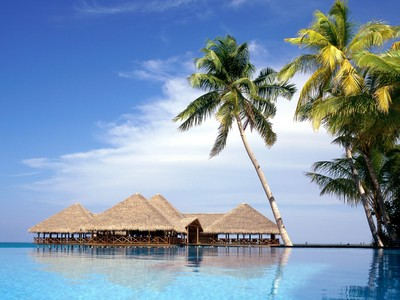
\includegraphics{input/p0-1-0}
\caption{p0-1-0}
\label{fig:p0-1-0}
\end{figure}

\item
\begin{enumerate}
\item PNG colored pictures has three channels of color, the Red, Green and Blue, the image (Figura \ref{fig:p0-2-a-0}) was obtained by swapping the values of the red channel with the blue channel, the green channel was left untouched.

\begin{figure}[ht]
\centering
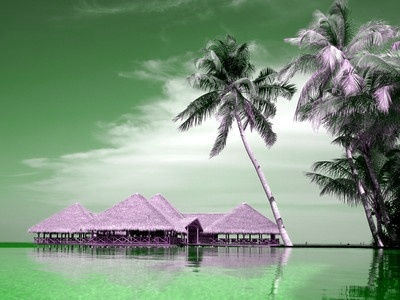
\includegraphics{output/p0-2-a-0}
\caption{p0-2-a-0}
\label{fig:p0-2-a-0}
\end{figure}

\item Monochrome or grayscale images are composed by one single channel which ranges from 0 to 255, thus all it takes to create a monochrome image from the green channel is to copy the green channel values, the result can be seen in Figura \ref{fig:img-green}

\begin{figure}[ht]
\centering
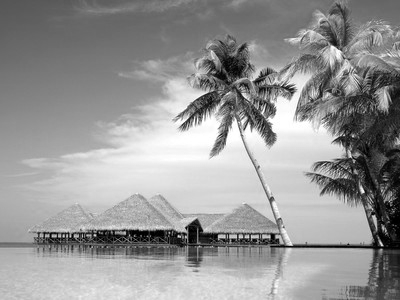
\includegraphics{output/img-green}
\caption{img-green}
\label{fig:img-green}
\end{figure}

\item Similar to the question above, except the red channel is used instead, result in Figura \ref{fig:img-red}

\begin{figure}[ht]
\centering
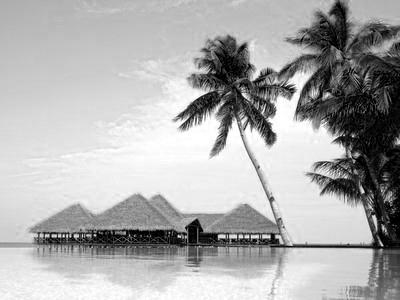
\includegraphics{output/img-red}
\caption{img-red}
\label{fig:img-red}
\end{figure}

\item 

The image made from the green channel looks more like what we expected, probably because of our nature sensibility to the green color, hence using it to create a image looks more aligned with what a human would expect.
\end{enumerate}

\item Q 3

\begin{figure}[ht]
\centering
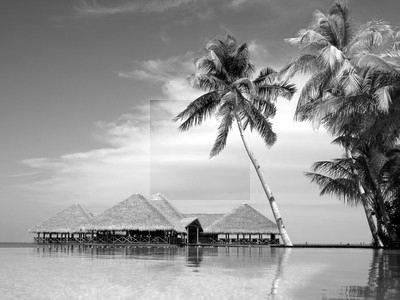
\includegraphics{output/p0-3-0}
\caption{p0-3-0}
\label{fig:p0-3-0}
\end{figure}

\begin{figure}[ht]
\centering
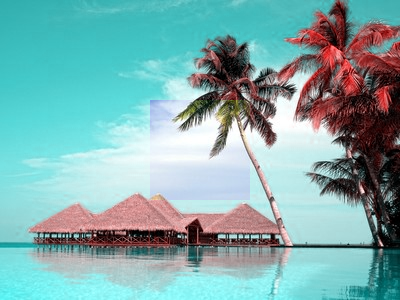
\includegraphics{output/p0-3-1}
\caption{p0-3-1}
\label{fig:p0-3-1}
\end{figure}

\item
\begin{enumerate}
\item Q 4a

\item Q 4b

\begin{figure}[ht]
\centering
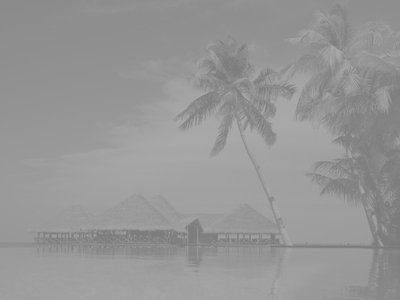
\includegraphics{output/p0-4-b-0}
\caption{p0-4-b-0}
\label{fig:p0-4-b-0}
\end{figure}

\item Q 4c
\end{enumerate}

\begin{figure}[ht]
\centering
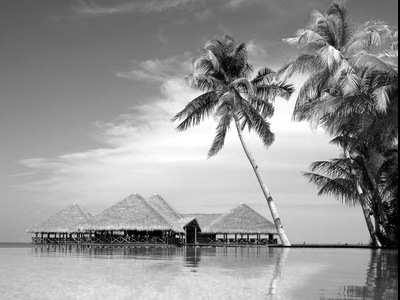
\includegraphics{output/p0-4-c-0}
\caption{p0-4-c-0}
\label{fig:p0-4-c-0}
\end{figure}

\begin{figure}[ht]
\centering
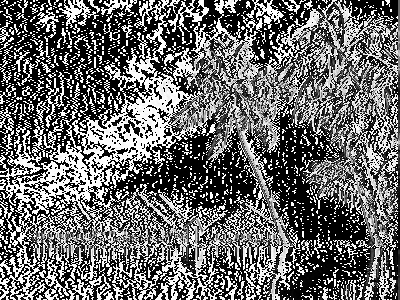
\includegraphics{output/p0-4-c-1}
\caption{p0-4-c-1}
\label{fig:p0-4-c-1}
\end{figure}

\item
\begin{enumerate}
\item Q 5a

\begin{figure}[ht]
\centering
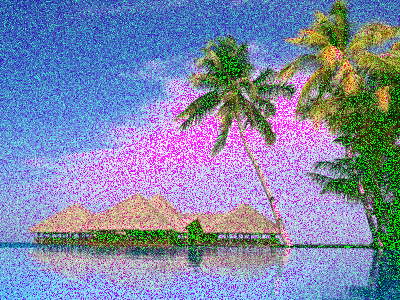
\includegraphics{output/p0-5-a-0}
\caption{p0-5-a-0}
\label{fig:p0-5-a-0}
\end{figure}

\item Q 5b

\begin{figure}[ht]
\centering
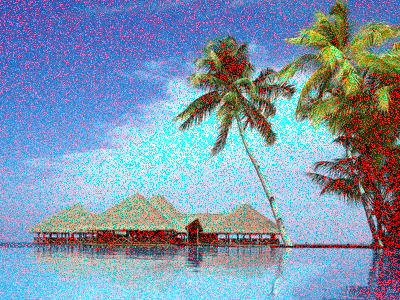
\includegraphics{output/p0-5-b-0}
\caption{p0-5-b-0}
\label{fig:p0-5-b-0}
\end{figure}

\item Q 5c
\end{enumerate}

\end{enumerate}
\end{document}

